\documentclass[10pt,conference]{IEEEtran}
\usepackage{diagbox}
\usepackage{graphicx}
\usepackage{amsmath}
\usepackage{amsfonts}
\usepackage{algpseudocode}
\usepackage{algorithm}
\usepackage{subfigure}
\usepackage{tikz}
\usepackage{epsfig}
\usepackage{cite}
\usetikzlibrary{shapes}
\usetikzlibrary{arrows,automata}
\usetikzlibrary{positioning}
\usetikzlibrary{patterns}
\usetikzlibrary{backgrounds}
\newtheorem{theorem}{Theorem}
\newtheorem{proposition}{Proposition}
\newtheorem{definition}{Definition}
\newtheorem{lemma}{Lemma}
\newtheorem{corollary}{Corollary}
\newtheorem{example}{Example}


\renewcommand{\ae}[1]{{\color{red}{#1}}}
\newcommand{\my}[1]{{\color{blue}{#1}}}
\newcommand{\old}[1]{{\color{green}{#1}}}
\newcommand{\pur}[1]{{\color{purple}{#1}}}

\begin{document}

\title{Towards Assured Machine Learning for CPS: Identify ``Unconfident'' Regions}
\author{
\IEEEauthorblockN{Xiaozhe Gu, Arvind Easwaran}
\IEEEauthorblockA{Nanyang Technological University, Singapore \\
Email: guxi0002@e.ntu.edu.sg, arvinde@ntu.edu.sg}
}
\maketitle


\begin{abstract} 
Machine learning (\emph{ML})  techniques are increasingly applied to decision-making and control problems in Cyber-Physical systems (CPS)  among which many are safety-critical, e.g., chemical  plants, robotics, autonomous vehicle, e.t.c.  Despite the benefit brought by ML techniques, they also raise safety issues because  1) most models produced by ML algorithms are not transparent and behave as  a block box and 2) the training data which plays a role as safety requirement is usually incomplete. An important  technique for  ML  to achieve safety  is ``Safe Fail'', i.e., a model rejects to predict and applies the backup solution when it has very low confidence in this prediction.  

Data-driven models produced by ML algorithms learn from training data and hence they are only as good as the examples that have learned.   As observed in many previous studies, feature space that lack of data generally have a much higher error rate than regions that contain sufficient  training samples~\cite{weiss2004mining}. Therefore, it is important  for CPS containing ML components  to classify such error-prone ``unconfident'' regions from ``confident'' regions such that predictions made in ``unconfident'' regions could be rejected.  In this paper, we propose an efficient tree based classifier to address this problem.  From the experiment results, we also show that ML models has much worse performance in the ``unconfident'' regions identified by our proposed technique. 

\end{abstract}


\section{Introduction}
In this section, we can talk about 
\begin{itemize}
    \item The trend of ML  in CPS and the need of safety AI.
    \item The safe fail technique, and the need to determine whether to reject predict.
\end{itemize}



\subsection{Background: Prediction with Uncertainty}
For classification problems,  the output of ML models is usually interpreted as model confidence in that prediction. For example,  output obtained at the end of the softmax layers of standard deep learning are often interpreted the predictive probabilities. If the obtained ``confidence'' level is very low, the models could select a reject option. A support vector machine (SVM) like classifier for classification with a reject option is proposed in~\cite{bartlett2008} for binary classification problems. For ensemble classifiers, the votes of base classifiers~\cite{varshney2013practical} will be used to determine whether to reject a prediction.  

The implicit assumption shared by classifiers is that ML models are most uncertain near the boundary between the different classes  and the distance from the decision boundary is inversely related to the confidence that the instance belong to that class. This is reasonable  to some extents because the decision boundaries learned by these models are usually located where a lot training samples belong to different classes overlap.   However, for feature space $\mathcal X$ that  contain few or no training samples at all,  then the learned the decision boundary may be completely based on an inductive bias, thereby containing much epistemic uncertainty~\cite{Attenberg:2015}. It is possible that an input instance that far from any training samples would be classified as some class  with very high probability~\cite{gal2016dropout}. 

Prediction uncertainty can also be obtained by Bayesian inference.  Bayesian probability theory provides a mathematically grounded tool to model the prediction uncertainty.   Gaussian process (GP)~\cite{seeger2004gaussian} is a  well known   probabilistic model and assumes that $p(f(\mathbf x_1), \ldots, f(\mathbf x_N ))$ is jointly Gaussian, with some mean $\mu(\mathbf x)$ and covariance $\Sigma(\mathbf x)$.  Given training samples $(\mathbf X,\mathbf y)$ and unobserved instance $\mathbf x_*$, the output $\mathbf f_*$ is also conditional Gaussian $p(\mathbf f_*|x_*,\mathbf X,\mathbf y)=\mathcal N(\mu_*,\sigma_*)$ where the standard deviation can be interpreted as the prediction confidence. GP is  computational intensive and has complexity $O(N^3)$, where N is the number of data.  Bayesian methods can also be applied to neural networks (NNs). Infinitely wide single hidden layer NNs with distributions placed over their weights converge to Gaussian processes~\cite{neal2012bayesian}. Variational inference~\cite{paisley2012variational,kingma2013auto} can be used to obtain  approximations for finite Bayesian neural networks. The  dropout  techniques in NNs can also be interpreted as a Bayesian approximation of  Gaussian process~\cite{gal2016dropout}. With all the good properties of Bayesian learning,  there are some  controversial aspects: 1) is its reliance on priors and  2) it is  computationally intensive.

The conformal prediction framework~\cite{Vovk:2005,vovk2009line} uses past experience to determine precise levels  of confidence in new predictions. Given a certain error probability $\epsilon$ requirement, it forms a prediction interval $[\overline{f(\mathbf x)},\underline{{f(\mathbf x)}}]$ for regression or a  prediction label set $\{\mbox{Label 1},\mbox{Label 2},\ldots \}$ for classification  so that the interval/set contains the actual prediction with probability $1-\epsilon$. However, its theoretically accuracy guarantee depends on the assumption that all the data are independent and identically distributed (in fact, i.i.d. assumption replaced by the weaker assumption of ``exchangeability'').  Besides, for regression problems, it tends to  produce prediction bands  whose width is roughly constant over the whole feature space~\cite{lei2018distribution}.





















\subsection{Motivation}
Data-driven  models are trained by ML learning algorithms using a subset of possible scenarios that could be encountered operationally.   Thus,  the models produced by ML algorithms  can only be as good as the examples that have learned.  However, the training set is usually incomplete and there is no guarantee that it is even representative of the space of possible inputs~\cite{ISO16}.  Previous study~\cite{weiss1995learning} has demonstrated that  feature space that lack of data generally have a much higher error rate.    

For example, Figure~\ref{fig:toy1} shows the decision boundary learned by a SVM classifier to predict the whether a wall-following  robot is turning right sharply.  The value in the contour map represents the probability learned by the classifier that the instance belong to class ``Sharp-Right-Turn''.  As we can observe, the training samples is not  representative of testing samples at all. However, the classifier still has relative high confidence in some regions where it has not well learned but lots of many testing samples locates. As a result, a lot of testing samples that belong to other classes are misclassified as ``Sharp-Right-Turn'', and accuracy for testing samples decreases to $66\%$ while the accuracy for training samples is almost $100\%$. In practice, safety-critical scenarios like traffic accidents are very rare and ML algorithms usually do not receive enough such training samples.


\begin{figure}[t]
\centering
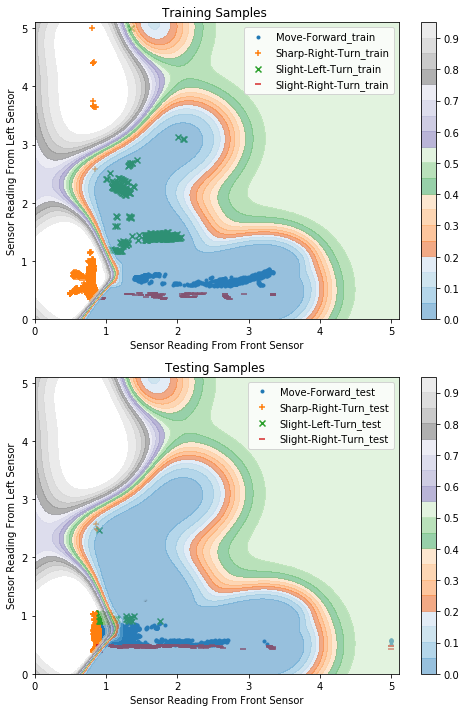
\includegraphics[width=0.45\textwidth]{FIG/toy1.png}
\caption{Wall-following navigation task with mobile robot SCITOS-G5 based on sensor readings from the front and left sensor~\cite{Dua:2017}.}
\label{fig:toy1}
\end{figure}


Therefore, it is very important to identify the feature space that the model is not well trained from that it does not receive enough training samples.

 % so that safety-critical systems with ML component could  REJECT OR GET MORE TRAINING SAMPLES

\noindent\textbf{Desired Characteristics}

\section{Evaluation}
\label{sec:evaluation}

In this section, we evaluate the effectiveness of our proposed technique by showing that different ML models (e.g., SVM, NNs, GP) have much higher loss (or error rates)  in the  identified ``unconfident'' regions.  However, one thing we should point out is  that, for classification problems,  ``unconfident'' regions do not always mean lower error rates. For example, Figure~\ref{fig:toy3} shows a binary classification problem where the decision boundary is a circle.  The SVM classifier has very high accuracy in the feature space far from the circle decision boundaries, even though it has learned very few or no training samples from these regions.  
\begin{figure}[t]
\centering
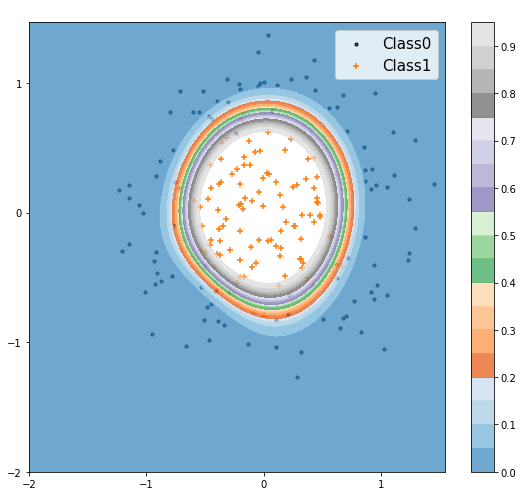
\includegraphics[width=0.4\textwidth]{FIG/toy3.png}
\caption{A binary classification toy  example}
\label{fig:toy3}
\end{figure}


\subsection{Classification Problems}

\subsubsection{The Navigation Task for Mobile Robot SCITOS-G5~\cite{Dua:2017}}




\subsection{Regression Problems}

\subsubsection{The Inverse Dynamics of a  SARCOS Robot Arm~\cite{SARCOS}}
The task is to map from a 21-dimensional input space (7 joint positions, 7 joint velocities, 7 joint accelerations) to the corresponding torque.


\begin{figure}[h]
\centering
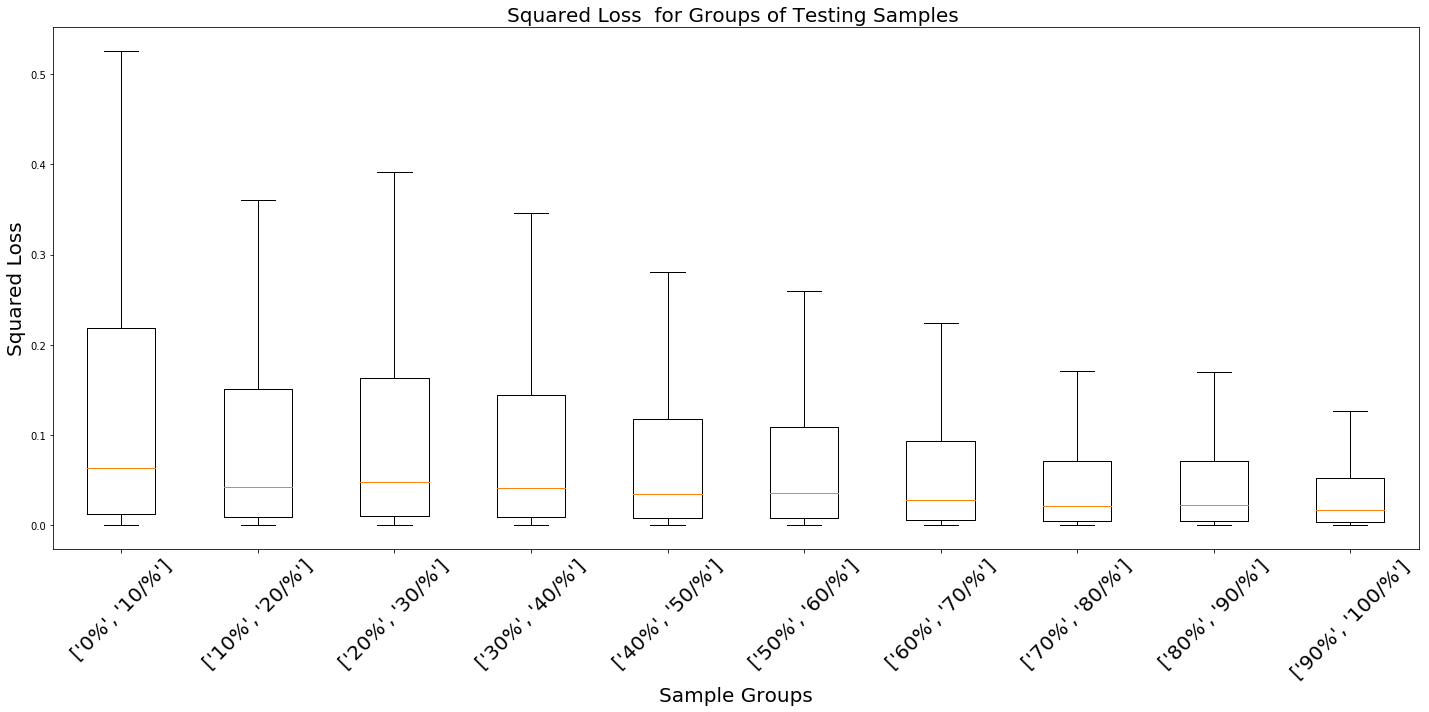
\includegraphics[width=0.5\textwidth]{PLT/sarcos_mlpbox.png}
\caption{SARCO: box plot of mean squared loss of NNs}
\label{fig:sarcos_mlpbox}
\end{figure}

\begin{figure}[h]
\centering
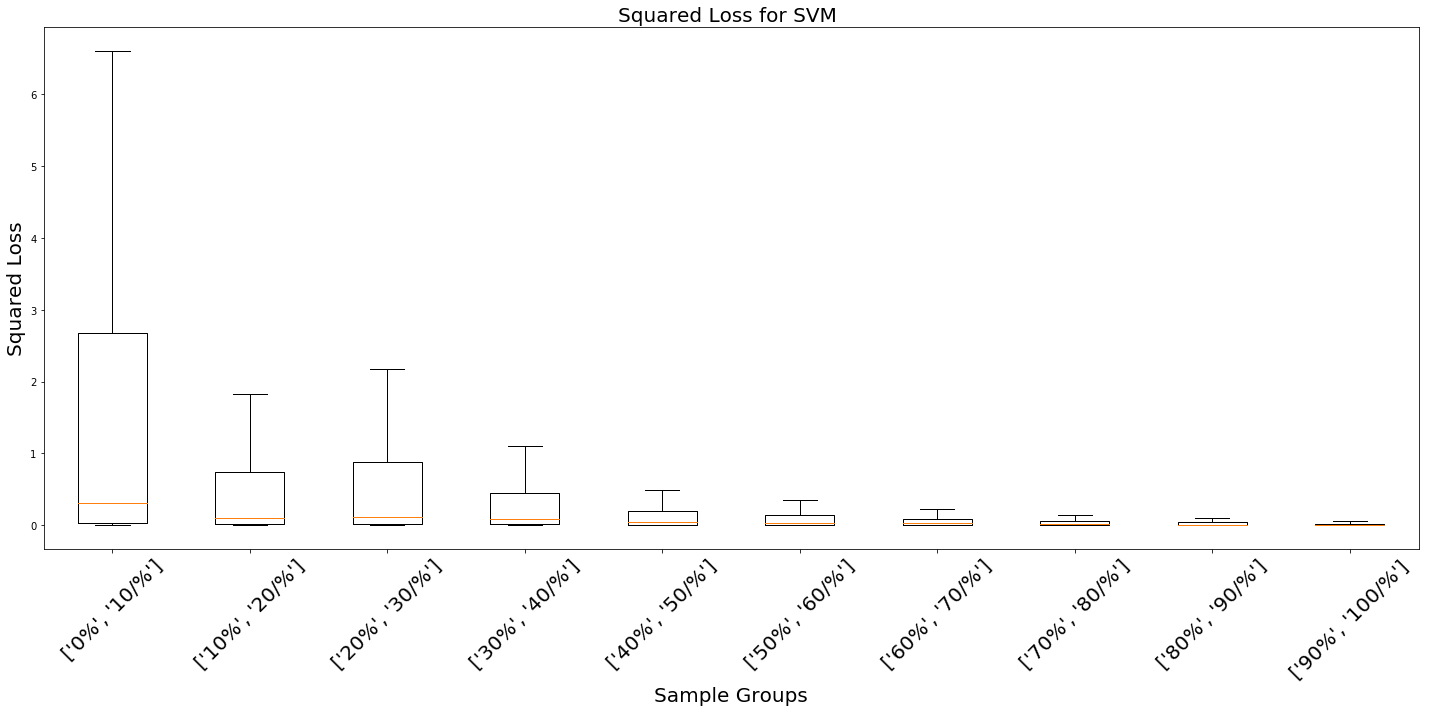
\includegraphics[width=0.5\textwidth]{PLT/sarcos_svmbox.png}
\caption{SARCO: box plot of mean squared loss of SVM}
\label{fig:sarcos_svmbox}
\end{figure}


\begin{figure}[h]
\centering
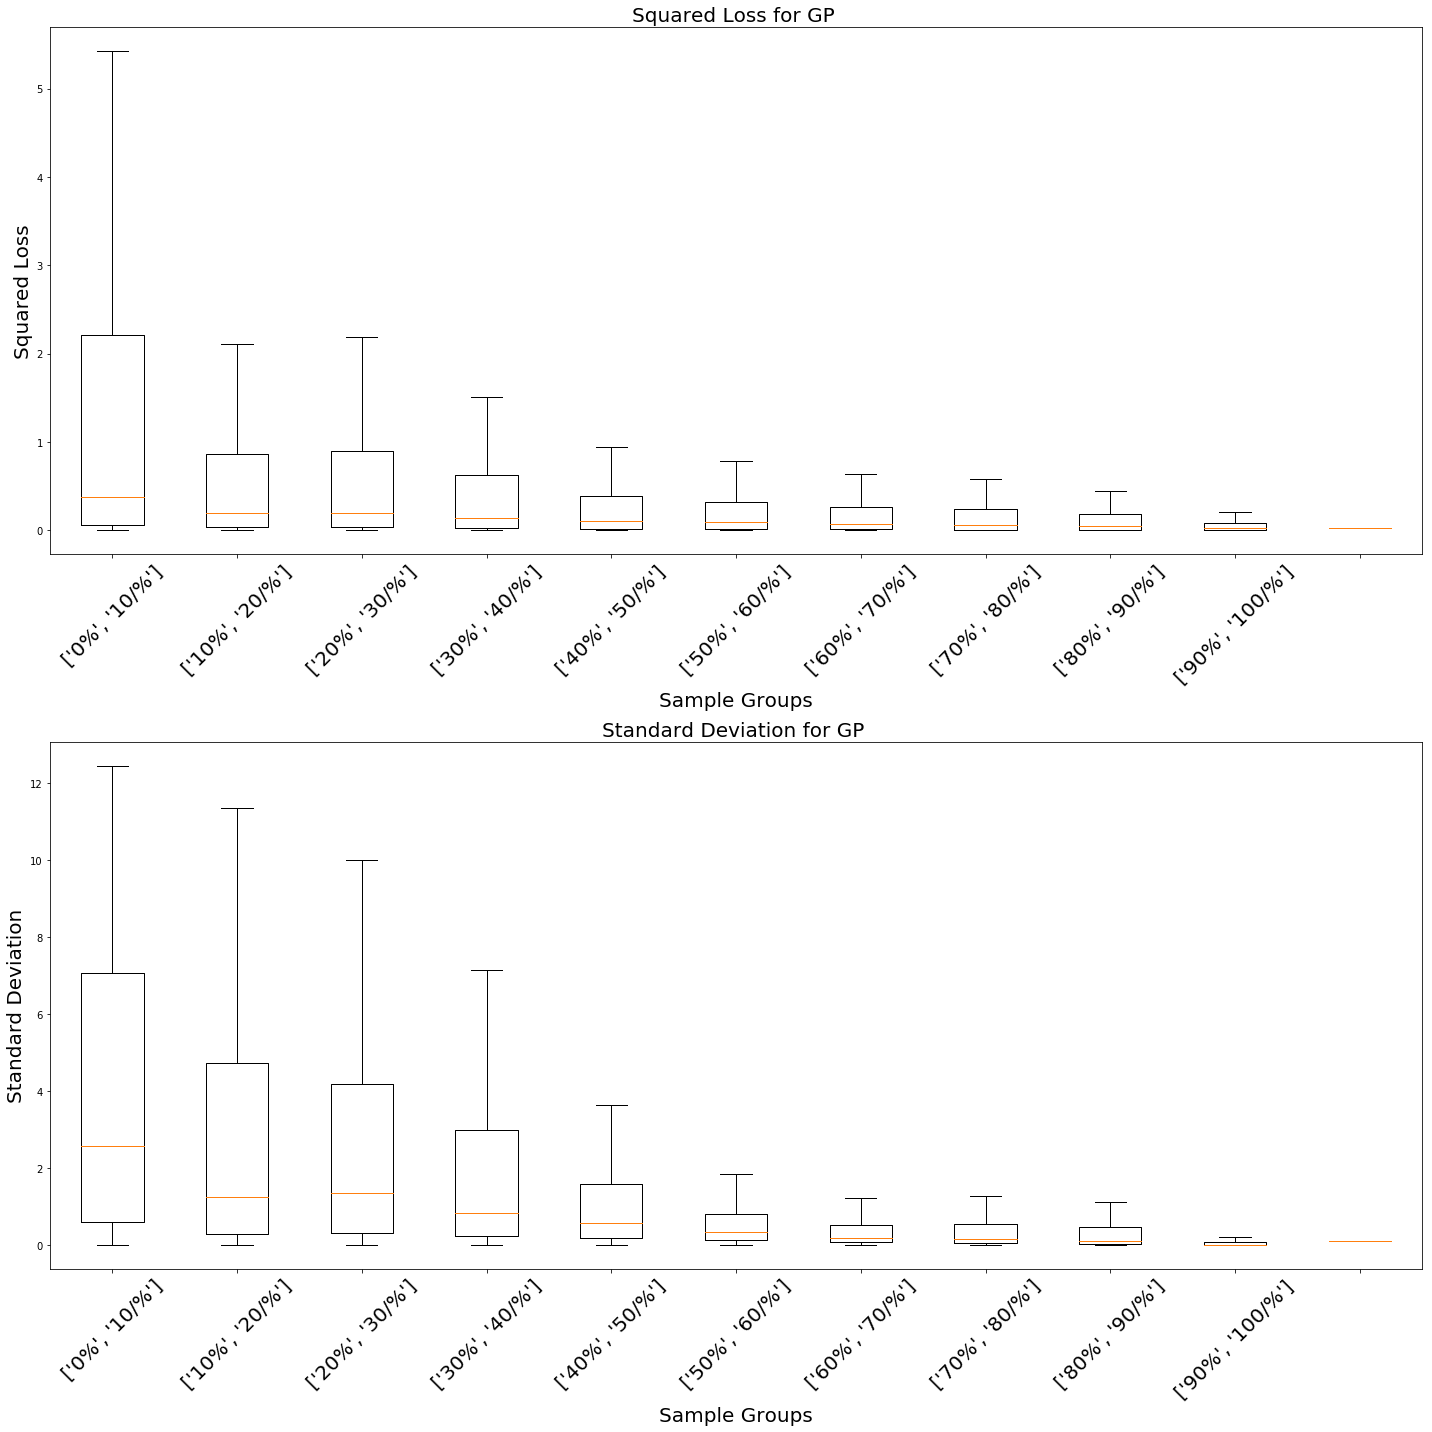
\includegraphics[width=0.5\textwidth]{PLT/sarcos_gpbox.png}
\caption{SARCO: box plot of mean squared loss and standard deviation of GP}
\label{fig:sarcos_gpbox}
\end{figure}


% In this example we consider learning the inverse dynamics of a seven degrees-of- freedom SARCOS robot arm1. The task is to map from a 21-dimensional input space (7 joint positions, 7 joint velocities, 7 joint accelerations) to the corresponding 7 joint torques. Following previous studies on this benchmark (see references in [14]) we only consider the mapping to the first of the seven torques, that is, we learn a function f : R21 → R. There are 44,484 training examples and 4,449 test examples. All 21 inputs xi have been standardized to have zero mean and standard deviation 1. The output y has zero mean. Results are given as standardized mean squared error (SMSE), which is the mean squared error on the test set divided by the variance of the target values in the test set. The normalization by the variance makes the error measure independent on the overall scale of the target.
% While in a real safety-related application the worst-case error should be consid- ered additionally to the mean error, here we solely use the SMSE to facilitate the comparison with previous studies.
% All methods described in the following were applied to this benchmark. The re- sulting SMSE accuracy is summarized in Table 1.



\section*{Acknowledgment}


\section{Conclusion}


\bibliographystyle{IEEEtran}
\bibliography{all}
\end{document}







